\documentclass[12pt,a4paper]{article}
\usepackage[utf8]{inputenc}
\usepackage[T1]{fontenc}
\usepackage{amsmath}
\usepackage{xcolor}
\usepackage{color}
\usepackage{pifont}
\everymath{\displaystyle}
\usepackage[francais]{babel}
\usepackage{fancyhdr}
\usepackage{fancybox}
\usepackage{hyperref}
\usepackage{graphicx}
\usepackage{wrapfig}

\usepackage{fancyhdr}
\usepackage[left=1.3cm,right=1.2cm,top=2cm,bottom=1.5cm]{geometry}
\usepackage{array}
\pagestyle{fancy}
\fancyhead[L]{Florentin Lespinasse~~~~~1STI2D4}
\fancyhead[C]{Devoir Maison}
\fancyhead[R]{08 Janvier 2020}
%\setlength{\parindent}{0}

\begin{document}
\begin{center}
        \shadowbox{\begin{large}
                \textcolor{black}{La Corrida}
        \end{large}}
    \end{center}
    \vspace{0.5 cm}
		\begin{presentation}
	\color{blue}	
	\noindent		\textbf{\underline{Histoire}}	\par
	\color{red}	
\textbf{	Francais} \par
					La corrida est un combat entre un homme et un taureau.
					Le but principal de l'homme est de mettre \`a mort le taureau par le biais de son \'ep\'ee.
					Le taureau peut \^etre exeptionnellement gr\^aci\'e.
					L'atraction se passe dans une ar\`ene pr\'evue \`a cet effet.
					Il se déroule dans un Anphitéhâtre avec au centre du sable et sur les côtées des gradins. \\
					Cela se d\'eroule en trois parties.\par 
				La premi\`ere partie, est d'affaiblir le taureau en le bl\'essant avec 3 paire de banderilles.
					L'homme qui fait cela, s'appelle le \textbf{Mantador}.
	 				Cela existe depuis l'antiquitée.
				les regles du 17e siecle ont cedes la place a de belles figures \par
		
	\color{black}	
\textbf{Espanol} \par
	Este atraction se pasa dentro una arena, un anfitheatro.
	Este espect\'aculo commencado desde la entig\"uedad.
	La Corrida es una lucha con un hombre y un toro. 
	El hombre dé muerte la toro por su estocade.
	El toro puede excepcionalmente perdonado.
	Un Corrida durante \textbf{dos Horas}.
	Durante estos tiempo, hay \textbf{tres Matador} contra \textbf{seis toro}.
	Hay \textbf{tres partes}.\\ 


		\end{presentation}


		\begin{dev}
		\noindent	\textbf{\underline{Développement}}\par
	\color{blue}	
		\item Le Matador \par
	\color{red}	
\textbf{	Francais} \par
		Ils peuvent etre plusieurs à jouer avec le taureau.
		Ils sont souvent habillé des couleurs qu'ils veullent mais doivent impérativement avoir la muleta rouge.
		Car cela favorise l'enervement du taureau\par
%		\begin{figure}[ht]
%		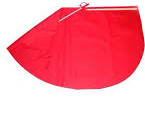
\includegraphics[scale=0.5]{1_images/muelta.jpeg}
%		\centering
%		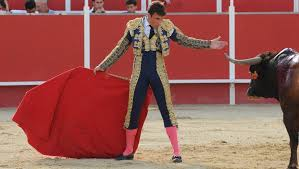
\includegraphics{1_images/matador.jpg}
%		\end{figure}	
%
%\begin{wrapfigure}[5]{l}{4cm}
%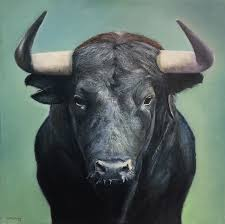
\includegraphics[scale=0.5]{1_images/toro_bravo.jpeg}
%\end{wrapfigure}
	\color{black}	
\textbf{Espanol} \par
	Pede estan varios hombres por juego con el toro
	Los Matadores, estan menudo con colores vivos pero deben hacer la muelta rojo.
	Porque esta colores exita el toro.



	\color{blue}	
		\item Le Taureau \par
	\color{red}	
\textbf{	Francais} \par

		Il vit pendant 4 ans dans la nature en libertée puis il est ensuite choisit pour son courrage et son agressivitée.
		Il pèses dans les 500 KG. Ce taureau est appelé \textit{toro bravo}.\par
	\color{black}	
\textbf{Espanol} \par
		El toro vide durante cuatro a\~nos en la natura.
		El es elige for su coraje y su agressividad.
		Es peso \textit{\textbf{Quinientos}}.
		Es toro esta tambien llamado \textit{Toro Bravo}.

	\color{blue}	
		\item Le déroulement \par
	\color{red}	
\textbf{	Francais} \par
		Cela se passe en 3 parties appelées \textbf{\textit{tercios}} \par
	\color{black}	
\textbf{Espanol} \par
		Este momente se passo en tres partes llama \textbf{\textit{tercios}}




	\color{blue}	
		\item Primo \par
	\color{red}	
\textbf{	Francais} \par
%\begin{wrapfigure}[8]{r}{10cm}
%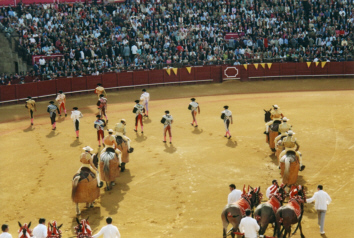
\includegraphics[width=10cm]{1_images/corrida-pst.jpg}
%\end{wrapfigure}

Cette phase marque l'entrée des picadors qui, à l'aide de piques, testent la bravoure de l'animal, mais également réduisent sa force, le calment et l'amènent à baisser la tête
		Il y a le matador, les picadores, et les peones.\par
	\color{black}	
\textbf{Espanol} \par
		La primera partes es la entrada de los picadores. 
		Con muchos picas, prueban la valencia de animal con reducen sus fuerza. 
		Hay el Matador, los picadores y los peones.\\\\\\


	\color{blue}	
		\item Segundo \par
	\color{red}	
\textbf{	Francais} \par
		est d'affaiblir le taureau en le bl\'essant avec 3 paire de banderilles.
		consiste à fatiguer le taureau.
		La seconde phase consiste à planter des 3 paires de banderilles entre les épaules du taureau.\par
	\color{black}	
\textbf{Espanol} \par
		La segundo partes, consiste en se debilita el toro en su plantarlo seis banderillas.
		 



	\color{blue}	
		\item tercio \par
	\color{red}	
\textbf{	Francais} \par
	C'est la mise a mort du taureau.
	Le matador effectu des passes de muelta pour monter encore une fois le courage du taureau.
	La mise a mort du taureau est effectue grace a son épée. c'est l'estocade 
	\color{black}	
\textbf{Espanol} \par
	El Matador juego con el toro gracias su Muelta para mostado el valencia de este toro.
	El matador da el glope fatal con su espada. 
	El momente se llama \textbf{\textit{Estocade}}
	Esta la muerte del toro.
	

		\end{dev}


\end{document}

